%%---%% Physics Lab Report Version 0.5 - 1.Maí 2021 %%---%%
% Höfundur/Author: Hákon Örn Árnason - hakona07 AT ru.is
% Viðhaldið af/Maintained by: Hákon Örn Árnason - hakona07 AT ru.is
%%%%%%%%%%%%%%%%%%%%%%%%%%%%%%%%%%%%%%%%%%%%%%%%%%%%%%%%%%%
% Credits to:
% Math template by Hlynur Arnarsson
% How to write text by Andrei Manolescu, Haraldur Auðunsson, Sigurður Ingi Erlingsson, version 050918
% Hákon Valur Haraldsson - figures and tables additions.
%%%%%%%%%%%%%%%%%%%%%%%%%%%%%%%%%%%%%%%%%%%%%%%%%%%%%%%%%%%

\documentclass{scrartcl}
% Skapalón frá Hlyni Arnórssyni
% Physics Version 0.2 - 10.Jan 2020
% ---------- Blaðsíðustillingar ---------- 
\usepackage{geometry}

\geometry{
	paper=a4paper, % letterpaper lika til
	top=2.5cm, % Top margin
	bottom=1cm, % Bottom margin
	left=2.5cm, % Left margin
	right=2.4cm, % Right margin
	headheight=0.75cm, % Header height
	footskip=1.5cm, % Space from the bottom margin to the baseline of the footer
	headsep=0.75cm, % Space from the top margin to the baseline of the header
	%showframe, % Uncomment to show how the type block is set on the page
}

% ---------- Íslenska ---------- 
\usepackage[T1]{fontenc}
\usepackage[utf8]{inputenc}
\usepackage[icelandic]{babel}

% ---------- Stærðfræðipakkar frá AMS ---------- 

\usepackage{amsmath, amsfonts, amsthm, amssymb} % Stærðfræðipakkar
\usepackage{braket, nicefrac} % fyrir mengi, brotabrot

% ---------- Fyrir SI Einingar ---------- 
\usepackage{siunitx}

% ---------- Listar/ númeringar ---------- 
\usepackage{enumitem, multicol}

% ---------- Fyrir innsetningu mynda ---------- 
\usepackage{graphicx, float} 
\usepackage{keystroke}
\usepackage{pgfplots}\usepgfplotslibrary{units}
\pgfplotsset{width=10cm,compat=1.9}
\usepackage{caption}
\newcommand{\source}[1]{\caption*{Source: {#1}} }

% ---------- Til að teikna/tekka myndir ---------- 
\usepackage{tikz}
\usepackage{tkz-euclide}
\usetikzlibrary{math}
\usepackage{fourier}
\usetikzlibrary{quotes,angles}
\usepackage{tkz-euclide}
\usetikzlibrary{calc}
\usetkzobj{all}
\usepackage[siunitx, nooldvoltagedirection]{circuitikz} %%<--- Circuit Diagrams/Rafrása myndir
\usepackage{csquotes}

%%%%%%%%%%%%%%%%%%%%%%%%%%
% ---------- Nýtt Matlab viðmót ---------- 
\usepackage{listings}
\usepackage{fancyvrb}

\def\lstbasicfont{\fontfamily{pcr}\selectfont\normalsize}
\definecolor{mygreen}{RGB}{28,172,0} 
\definecolor{mylilas}{RGB}{170,55,241}
\lstset{language=Matlab,%
	basicstyle={\lstbasicfont},
	breaklines=true,%
	morekeywords={matlab2tikz},
	keywordstyle=\color{blue},%
	morekeywords=[2]{1}, keywordstyle=[2]{\color{black}},
	identifierstyle=\color{black},%
	stringstyle=\color{mylilas},
	commentstyle=\color{mygreen},%
	showstringspaces=false, %without this there will be a symbol in the places where there is a space
	numbers=left,%
	numberstyle={\tiny \color{black}},% size of the numbers
	numbersep=5 pt, % this defines how far the numbers are from the text 
	inputencoding=latin1,
	backgroundcolor = \color{gray!3},
	framexleftmargin= -1 mm,
	frame=none,
	rulesepcolor=\color{blue!30},
	extendedchars=true,
	emph={logical},emphstyle=\color{blue},	
	emph={all,equal, minor, on, off, long, short, bank, rat},emphstyle=\color{mylilas},	
}
\renewcommand\lstlistingname{\textsc{Matlab}}%

\usepackage{tcolorbox}
\tcbuselibrary{skins}
% ---------- Hérna vel ég stillingar fyrir ramma sem ég skýri matlabUT
\tcbset{matlabUT/.style={
		enhanced,
		colback=gray!1,
		colframe=gray!30,
		title=Command Window,
		arc=0mm,
		coltitle=black,
		center title, 
		title style={top color=white, bottom color = gray!30},
		grow to left by= -3 mm,
		left= 4 mm,
		grow to right by=0.5mm,
		colupper = gray!70!black
}}

%  ---------- Les inn textaskra sem inniheldur niðurstöður úr Command Window
\newcommand{\CommandWindow}[1]{\begin{tcolorbox}[matlabUT]
		\VerbatimInput{#1}
\end{tcolorbox}}


%%%%%%%%%%%%%%%% Matlab endar %%%%%%%%%%%%%%%%%%%%%%%%%%%%%%%%%%%%%%%%

%%%%% Geogebra  %%%%%%%%%%%%%%%%%%%%%%%%%%%%%%%%%%%%%%%%%%%%%%%%%
% ---------- Nokkur tól í GeoGebru, smíða einnig skurðtólið ---------- 

\newcommand{\Punktur}{% Punktur í GeoGebru
	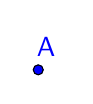
\begin{tikzpicture}[scale = 2]
	\draw
	(0,0) coordinate(A)
	(0.05,0.025) coordinate(pos)
	node[blue, anchor = south] {$\mathsf{A}$}  
	[blue,fill](A) circle(0.85pt); 
	\draw      [color = black](A) circle(0.9pt);
	\end{tikzpicture}
}
\newcommand{\Linustrik}{%  Strik, segment
	
\begin{tikzpicture}[scale = 0.4]
	\draw
	(0,0) coordinate(A)
	(1,0.7) coordinate(B)
	[line width = 1pt, blue](A)--(B);
	\draw[blue, fill](A) circle(4pt);
	\draw[blue, fill](B) circle(4pt);
	\end{tikzpicture}	
}

\newcommand{\Lina}{% bein lína, hægt að framlengja að vild
	
\begin{tikzpicture}[scale = 0.5]
	\draw
	(0,0) coordinate(A)
	(1,0.7) coordinate(B)
	[line width = 1pt, blue](A)--(B);
	\draw[blue, fill](0.25,0.18) circle(3pt);
	\draw[blue, fill](0.74,0.53) circle(3pt);
	\end{tikzpicture}	
}
\newcommand{\Halflina}{% við smíð á hornum
	
\begin{tikzpicture}[scale = 0.4]
	\draw
	(0,0) coordinate(A)
	(1,0.7) coordinate(B)
	[line width = 1pt, blue](A)--(B);
	\draw[blue, fill](A) circle(3pt);
	\draw[blue, fill](0.65,0.45) circle(3pt);
	\end{tikzpicture}	
	
}

\newcommand{\GeoO}{
	\begin{tikzpicture}[rotate=30,transform canvas={scale=0.18},yshift=7mm]
	\def\xrad{0.7}
	\def\yrad{0.58}
	\definecolor{GeogebraLitur}{rgb}{0.6,0.60,100}
	\tikzset{hnutur/.style={shape=circle, line width=0.7mm,color=black, fill=GeogebraLitur, scale=0.8, draw}} % 0.8
	\draw[ color = gray!70!black, line width=1.3mm] (0,0) circle[x radius = \xrad cm, y radius = \yrad cm];
	\def\n{5}
	\foreach \k in {1,...,\n}
	\node at ({360/\n*\k-10}:\xrad cm and \yrad cm)[hnutur] {};
	%	node[pos=1,hnutur]{} ;
	\end{tikzpicture}
}
\newcommand{\Geogebra}{{\color{gray!70!black}\textsf{Ge}\ \GeoO\textsf{Gebra }}}


%%%%%%%%%%%%%%%%%%%%%%%%%% Hyperlink References %%%%%%%%%%%%%%%%%%%%%%%%%%%
\usepackage{hyperref}

% ---------- Skrá fyrir myndir ---------- 
\graphicspath{{graphics/}{Graphics/}{./}}
% ---------- Skrá fyrir heimildir ---------- 
\usepackage[style=ieee]{biblatex}
\addbibresource{bibliography.bib}

\begin{document}

%% --- Titil síða / Title page --- %%
\begin{titlepage}
	\centering
	
\includegraphics[width=0.3\textwidth]{ru-logo-1.pdf}\par\vspace{1cm} %<-- RU Logo
	{\scshape\LARGE Háskólinn í Reykjavík \par} %<-- Nafn háskólans (Háskólinn í Reykjavík / Reykjavik University)
	\vspace{1cm}
	{\scshape\Large Physics Lab Report\par} %<-- Áfanga titill / Class or course title
	\vspace{1.5cm}
	{\huge\bfseries How to write One\par} %<-- Titill Skýrslu / Title of Report
	\vspace{2cm}
	{\Large\itshape Nemandi 1}\par %<-- Nafn nemanda / Name of student
	\texttt{ElskarEðl@ru.is}\par %<-- t-póstfang / e-mail
	\vspace{0.5cm}
	{\Large\itshape Nemandi 2}\par %<-- Nafn nemanda / Name of student
	\texttt{Gerðiekkert@ru.is}\par %<-- t-póstfang / e-mail
	\vfill
	supervised by\par %<-- (Umsjón höfðu / supervised by)
	Teacher \& Assistant %<-- Nafn kennara og aðstoðarkennara í tilraun / Name of Lab Teacher and TA
	\vfill

% Bottom of the page
	{\large \today\par}
\end{titlepage}

%% --- Titil síða endar / Title page ends --- %%

\section{Introduction} %<--  Inngangur / Introduction

In this section of the report you explain the basic physical phenomenon, the principle(s), and the basic equations.
All notations or symbols used in the equations will be explained.
Using one or two figures to make the explanations clear is highly recommended.
You also state briefly what you want to do or test in this lab/experiment\cite{anarticle, thesis, report, conv, unpub, notpub, notpub}.
Do not copy-paste from the written documentation created for you.
Use your own understanding.
Imagine you are an expert working in a professional lab and you write a report for your clients or for your collaborators who are asking you to do measurements on their samples or materials.
So you explain to them the basics of the experiment and the measurements.
It is assumed that they already have some general knowledge, but they are not necessarily experts in your field.
The recommended size of this section is about one page including figures.

\begin{equation}\label{eu_eqn}
e^{\pi i} + 1 = 0
\end{equation}

The beautiful equation \ref{eu_eqn} is known as the Euler equation\cite{collection}

\section{Methods} %<--  Aðferð / Methods -- Yfirkafli

Here you explain methods used in the experiment\cite{bookseries}.
Statistical methods, measurement methods...

\subsection{Equipment and setup} %<-- Uppsetning og tæki / Equipment and setup -- undirkafli

Here you explain the equipment you used and the experimental setup.
Mention the instruments or the accessories used.
Do not list up all the tools, but only the most important.
Pictures might be very helpful.

% --- Gerð rafrásamynda
% --- How to make Circuit diagrams pictues
% https://www.overleaf.com/learn/latex/LaTeX_Graphics_using_TikZ:_A_Tutorial_for_Beginners_(Part_4)%E2%80%94Circuit_Diagrams_Using_Circuitikz
\begin{figure}[h]
    \centering
        \begin{circuitikz}
        \draw
        (0,0) to[battery] (0,4)
          to[ammeter, i_=2<\milli\ampere>] (4,4) 
          to[vR] (4,0) -- (3.5,0)
          to[lamp, *-*] (0.5,0) -- (0,0)
        (0.5,0) -- (0.5,-2)
          to[voltmeter, l=3<\kilo\volt>] (3.5,-2) -- (3.5,0)
        ;
        \end{circuitikz}
        \caption{(Example caption) Some description about the diagram.}
        \label{fig:Circuit_diag}
\end{figure}


\subsection{Procedure} %<-- Framkvæmd / Procedure -- Undirkafli

Describe the most important steps of the work.
Do not go into too many details, like: “we opened the Capstone software and clicked Start”, or “we turned on the power source”. \cite{abook} %<-- heimild
Such information is irrelevant for your clients or collaborators.
Again, do not copy-paste from the description of the teacher.
Explain your work such that the readers will understand what you did and will trust you.
In general half a page should be sufficient here, but you can write more, depending on the complexity.
You can include more technical details like limitations of the equipment, or improvements that you made, or other methodological aspects.

\section{Results and Discussion} %<-- Niðurstöður og umræða / Results and Discussion

Describe the data collection briefly and put the data tables and figures in context.
In experiments when an electric circuit is studied the circuit and the meters used should be shown in the report.
Data tables.
Show the data tables.
All tables should be numbered (like Table n), have a title and include a brief description.
This description should be on top of the table. Of course, if you have thousands of numbers do not show all, but only the most important.
Always mention the physical units used.

% --- Tafla / Table 
\begin{table}[ht] %<-- [ht] stýrir staðsetningu miðað við texta.
    \centering
    \begin{tabular}{llr} %<-- "llr" stýrir útliti töflu
\hline
\multicolumn{2}{c}{Item} \\ %<-- 
\cline{1-2}
Animal    & Description & Weight (\si{\gram}) \\
\hline %<-- býr til þverlínu
Gnat      & per gram    & \SI{13.65}{\gram}      \\ %<-- & aðgreinir dálka
          & each        & \SI{0.01}{\gram}       \\ %<-- \\ gerir nýja línu
Gnu       & stuffed     & \SI{92.50}{\gram}      \\
Emu       & stuffed     & \SI{33.33}{\gram}      \\
Armadillo & frozen      & \SI{8.99}{\gram}       \\
\hline
\end{tabular}
    \caption{Results of measuring different types of frozen perishables.
    The description tells how each item is prepared.}
    \label{tab:my_label}
\end{table}

\textbf{\textit{Graphs.}} 

Often the graphs are the most important information of the work.
Whether you do a graph with the computer or by hand, do it with great care.
A graph contains a lot of information in a few cm2.
Graphs should be numbered (like Graph n), have a title and include a brief description.
This description should be below the graph itself. Label the axes the quantities shown and the units.
Some software (like Excel) do not have convenient default options for graphs:
grid-lines may be shown in one direction only, the displayed intervals might be much larger than the relevant intervals, etc. 
Find the convenient settings, do not accept the default if it is not good enough.
Use the whole graph area to show your data. Often you have to create either a straight line or another curve through the data points.
If you cannot do it with the computer, just print the graph and do it by hand.
Make sure that individual data points stand out clearly, they are your measurements.


\begin{figure}[h] %<-- [h] stýrir staðsetningu á mynd.
    \centering
    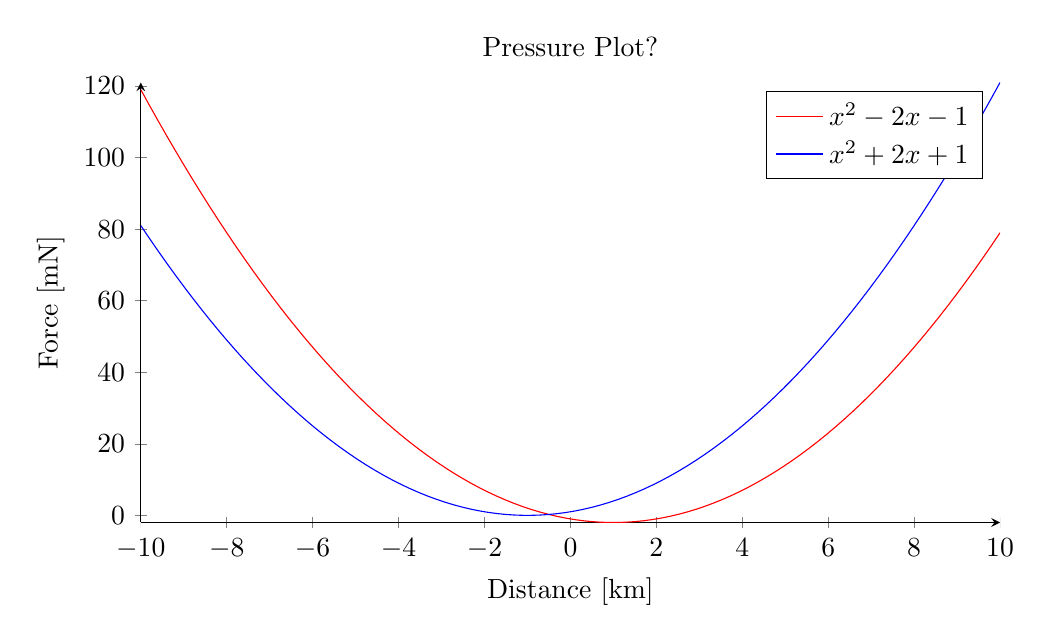
\begin{tikzpicture}
    \begin{axis}[
        height=0.2\paperheight,
        width=0.9\linewidth,
        scale only axis,
        title = Pressure Plot?,
        axis lines = left,
        x SI prefix=kilo,
        x unit=m,
        y SI prefix=milli,
        y unit=N,
        xlabel=Distance,
        ylabel=Force,
     ]
    %Below the red parabola is defined
    \addplot [
        red,
        domain=-10:10, 
        samples=100, 
    ]
    {x^2 - 2*x - 1}; %<-- hægt er að setja inn gagnaskrá í stað jöfnu ( væri þá sett í "Data_Files" og vísað síðan í hana hér )
    \addlegendentry{$x^2 - 2x - 1$}
    %Here the blue parabloa is defined
    \addplot [
        blue,
        domain=-10:10, 
        samples=100,
        ]
        {x^2 + 2*x + 1};
    \addlegendentry{$x^2 + 2x + 1$}
     
    \end{axis}
\end{tikzpicture}
    \caption{(Example caption) Figure shows how the system pressure in [Pressure(\si{\newton\metre})]changes with time for two cases.
    Blue is the first and red is the second case.}
    \label{fig:merkimiði_myndar}
\end{figure}

\textbf{\textit{Calculations.}} 

Show your calculations.
Show clearly the units you used for all physical quantities.
Here you show the error/uncertainty analysis.
Pay attention to the significant digits of the final results:
as a rule the uncertainty will be shown with only one significant digit and the main result with the last significant digit corresponding to the uncertainty.\\
Examples: 2.41±0.03 or 6.5±0.2 and not 2.412367±0.02698 nor 6.4±0.16.

\textbf{\textit{Discussion.}} 
Discuss briefly your results, how well they fit some model, theory or other data.

\section{Summary and Conclusions} %<-- Samantekt og niðurstöður / Summary and Conclusions

It is very important to have a clear, short, and informative summary of all the important results.
It can be a short table or a list, and possibly one or two short comments or explanations.
You have to understand that your clients or collaborators may not have time to read the whole report as soon as they see it, but they need the results or the conclusions immediately.
This is a typical situation in real life.
Some readers will look only at the last section first, and only later to the whole report.
That’s why in this final section you answer the initial question(s) or respond to what you wanted to do, as stated in the Introduction\cite{abook}.

\begin{figure}[h]
    \centering
    \includegraphics[scale=0.2]{Classical_laboratory_methods_in_microbiology.jpg}
    \caption{Dæmi um lélega samvinnu; allir að horfa á einn sem ætlar sér að gera góða skýrslu. ( Frá öðru sjónarhorni; allir að læra af þeim sem kann eitthvað fyrir sér)}
    \caption*{Source: \href{https://commons.wikimedia.org/wiki/File:Classical_laboratory_methods_in_microbiology.jpg}{Photo} by Dariusz Bartosik / \href{https://creativecommons.org/licenses/by/2.0/}{CC BY}}
    \label{fig:Þessi_mynd}
\end{figure}

\textbf{\textit{Final recommendations:}} 
The length of the report is not fixed.
In general it should be between 4 and 6 pages, but it may vary depending on the number of graphs and tables included.
Language can be English or Icelandic, at your choice.
This description is an addition and clarification to “Skýrslur og ritgerðir” as published by the School of Science and Engineering, and is specific to physics lab reports.

\newpage
\printbibliography

%------ To create Appendix with additional stuff -------%
%\newpage
%\appendix
%\section{Appendix/Fylgi gögn}
%Put data files, CAD drawings, additional sketches, etc.

\end{document}
